% !TEX spellcheck = en_US



% ~~~~~~~~~~~~~~~~~~~~~~~~~~~~~~~~~~~~~~~ V
% (NC) 2026 Haluk Bingol
% github.com/halukbingol/LaTeX-Templates
%
% Licensees may copy, distribute, display, and perform the work and make derivative works 
% and remixes based on it only for non-commercial purposes. 
% ~~~~~~~~~~~~~~~~~~~~~~~~~~~~~~~~~~~~~~~ A




% =====================================================================
%  Git -- Sophomore Level: Branches, Remotes and Teamwork
%  ---------------------------------------------------------------------
%  Built on hblib/Template/hblibTemplate.tex with the libraries in ../../hblib/.
%  Programs and their real outputs are in codeoutput/:
%     codeoutput/<Name>.java  a program (classes without main() are only compiled)
%     codeoutput/<Name>.sh    a terminal session, run in a copy of codeoutput/<Name>/
%     codeoutput/<Name>.txt   what it printed, made by:  bash run_examples.sh
% =====================================================================

\documentclass[aspectratio=169,10pt,compress]{beamer}

% ~~~~~~~~~~~~~~~~~~~~~~~~~~~~~~~~~~~~~~~~~~~~~~~~~~~~~~~~~~~~~~~~~ V hblib
	\usepackage{../../hblib/hblibPresentation} % lib presentation: theme, i/N, \hSection, algorithm2e, ...
	\usepackage{../../hblib/hblibCodeoutput} % lib code + output: \lstcode, \lstterminal, ...
	\usepackage{../../hblib/hblibDatastructures} % lib data structures: \hString, \hStack, \hQueue
% ~~~~~~~~~~~~~~~~~~~~~~~~~~~~~~~~~~~~~~~~~~~~~~~~~~~~~~~~~~~~~~~~~ A hblib


% xcolor, array (and the L{width} column), listings, tikz and algorithm2e come from the hblib libraries
\usepackage[T1]{fontenc}
\usepackage{lmodern}
\usepackage{booktabs}

\newcommand{\win}{\textbf{Windows}}
\newcommand{\mac}{\textbf{macOS}}

% algorithm2e set-up (the package is loaded by hblibPresentation)
\SetAlCapFnt{\small}
\SetAlCapNameFnt{\small}
\SetKwProg{Fn}{function}{}{end}
\SetKw{KwError}{error}

% ---------------------------------------------------------------------
\title{Git}
\subtitle{Sophomore Level: Branches, Remotes and Teamwork}
\author[Bingol]{Haluk O. Bingol}

\institute[FCIS]{
    Faculty of Computer and Information Sciences\\
    Yeditepe University
}
\date{
	{\tiny \hbTimeStamp}
}

\begin{document}




% ~~~~~~~~~~~~~~~~~~~~~~~~~~~~~~~~~~~~~~ V frm
\begin{frame}[t,fragile]
  \titlepage
\end{frame}
% ~~~~~~~~~~~~~~~~~~~~~~~~~~~~~~~~~~~~~~ A frm




% ~~~~~~~~~~~~~~~~~~~~~~~~~~~~~~~~~~~~~~ V frm
\begin{frame}[t,fragile] \frametitle{Outline}
  \begin{columns}[T]
    \begin{column}{0.48\textwidth}
      \tableofcontents[sections={1-4}, hideallsubsections]
    \end{column}
    \begin{column}{0.48\textwidth}
      \tableofcontents[sections={5-7}, hideallsubsections]
    \end{column}
  \end{columns}
\end{frame}
% ~~~~~~~~~~~~~~~~~~~~~~~~~~~~~~~~~~~~~~ A frm

% ~~~~~~~~~~~~~~~~~~~~~~~~~~~~~~~~~~~~~~ V
\hSection[Setup]{The Setting}
% ~~~~~~~~~~~~~~~~~~~~~~~~~~~~~~~~~~~~~~ A




% ~~~~~~~~~~~~~~~~~~~~~~~~~~~~~~~~~~~~~~ V frm
\begin{frame}[t,fragile] \frametitle{A team, a server, two laptops}
  \begin{columns}[T]
    \begin{column}{0.5\textwidth}
      \begin{center}
      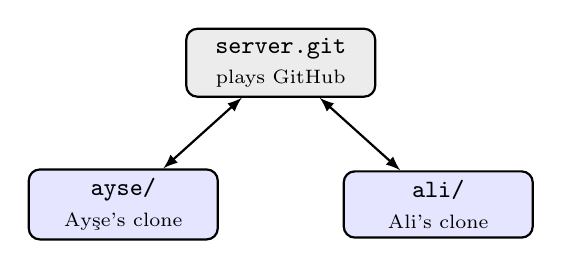
\begin{tikzpicture}[repo/.style={draw, thick, rounded corners, minimum width=2.4cm, minimum height=0.8cm, align=center, font=\small}]
        \node[repo, fill=gray!15] (s) at (0,0) {\texttt{server.git}\\ \scriptsize plays GitHub};
        \node[repo, fill=blue!10] (a) at (-2,-1.8) {\texttt{ayse/}\\ \scriptsize Ayşe's clone};
        \node[repo, fill=blue!10] (b) at (2,-1.8) {\texttt{ali/}\\ \scriptsize Ali's clone};
        \draw[latex-latex, thick] (a) -- (s);
        \draw[latex-latex, thick] (b) -- (s);
      \end{tikzpicture}
      \end{center}
    \end{column}
    \begin{column}{0.46\textwidth}
      \begin{itemize}\small
        \item Every session starts with a \textbf{bare} repository \texttt{server.git} and two clones, made by hidden set-up lines.
        \item A bare repository has no working tree: only the history. GitHub stores your repositories like this.
        \item With GitHub, only the URL changes: \texttt{git clone https://github.com/USER/shop.git}.
        \item Ali and Ayşe have their own names; the clock is fixed, so hashes repeat.
      \end{itemize}
    \end{column}
  \end{columns}
\end{frame}
% ~~~~~~~~~~~~~~~~~~~~~~~~~~~~~~~~~~~~~~ A frm

% ~~~~~~~~~~~~~~~~~~~~~~~~~~~~~~~~~~~~~~ V
\hSection[Feature]{Feature Branches and Pull Requests}
% ~~~~~~~~~~~~~~~~~~~~~~~~~~~~~~~~~~~~~~ A




% ~~~~~~~~~~~~~~~~~~~~~~~~~~~~~~~~~~~~~~ V frm
\begin{frame}[t,fragile] \frametitle{A feature branch from start to finish}
  \begin{columns}[T]
    \begin{column}{0.49\textwidth}
      \lstterminal[basicstyle=\ttfamily\tiny, lastline=14]{codeoutput/Feature.txt}
    \end{column}
    \begin{column}{0.49\textwidth}
      \lstterminal[basicstyle=\ttfamily\tiny, firstline=15]{codeoutput/Feature.txt}
    \end{column}
  \end{columns}

  \vspace{0.1em}
  \small
  \texttt{push -u} creates the branch on the server and links it (\emph{upstream}). On GitHub you would now open a \textbf{pull request};
  \texttt{merge -{}-no-ff} here does what its ``Merge'' button does.
\end{frame}
% ~~~~~~~~~~~~~~~~~~~~~~~~~~~~~~~~~~~~~~ A frm




% ~~~~~~~~~~~~~~~~~~~~~~~~~~~~~~~~~~~~~~ V frm
\begin{frame}[t,fragile] \frametitle{Pull requests}
  \begin{columns}[T]
    \begin{column}{0.5\textwidth}
      \begin{enumerate}\small
        \item push the branch
        \item open a pull request (PR) \texttt{feature/discount} $\to$ \texttt{main}
        \item CI runs the tests on the branch
        \item teammates review and comment line by line
        \item push more commits to fix the comments: the PR updates itself
        \item merge, delete the branch
      \end{enumerate}
    \end{column}
    \begin{column}{0.46\textwidth}
      \begin{block}{Three merge buttons on GitHub}
        \small
        \begin{itemize}
          \item \textbf{Create a merge commit}: \texttt{merge -{}-no-ff}
          \item \textbf{Squash and merge}: all PR commits become one (\texttt{merge -{}-squash})
          \item \textbf{Rebase and merge}: commits are replayed on \texttt{main}, no merge commit
        \end{itemize}
      \end{block}
      \small Protect \texttt{main}: no direct pushes, at least one review, green CI.
    \end{column}
  \end{columns}
\end{frame}
% ~~~~~~~~~~~~~~~~~~~~~~~~~~~~~~~~~~~~~~ A frm




% ~~~~~~~~~~~~~~~~~~~~~~~~~~~~~~~~~~~~~~ V frm
\begin{frame}[t,fragile] \frametitle{Squash: many small commits become one}
  \begin{columns}[T]
    \begin{column}{0.49\textwidth}
      \lstterminal[basicstyle=\ttfamily\tiny, lastline=13]{codeoutput/Squash.txt}
    \end{column}
    \begin{column}{0.49\textwidth}
      \lstterminal[basicstyle=\ttfamily\tiny, firstline=14]{codeoutput/Squash.txt}
    \end{column}
  \end{columns}

  \vspace{0.1em}
  \small
  \texttt{-{}-squash} stages the combined change without making a merge commit; the branch's ``wip'' commits stay out of \texttt{main}'s history.
\end{frame}
% ~~~~~~~~~~~~~~~~~~~~~~~~~~~~~~~~~~~~~~ A frm

% ~~~~~~~~~~~~~~~~~~~~~~~~~~~~~~~~~~~~~~ V
\hSection[Sync]{Keeping in Sync}
% ~~~~~~~~~~~~~~~~~~~~~~~~~~~~~~~~~~~~~~ A




% ~~~~~~~~~~~~~~~~~~~~~~~~~~~~~~~~~~~~~~ V frm
\begin{frame}[t,fragile] \frametitle{Push rejected: someone pushed first}
  \begin{columns}[T]
    \begin{column}{0.49\textwidth}
      \lstterminal[basicstyle=\ttfamily\tiny, lastline=17]{codeoutput/Rejected.txt}
    \end{column}
    \begin{column}{0.49\textwidth}
      \lstterminal[basicstyle=\ttfamily\tiny, firstline=18]{codeoutput/Rejected.txt}
    \end{column}
  \end{columns}

  \vspace{0.1em}
  \small
  Git never overwrites the server's commits. \texttt{pull} = \texttt{fetch} + \texttt{merge}: here a merge commit, then the push succeeds.
\end{frame}
% ~~~~~~~~~~~~~~~~~~~~~~~~~~~~~~~~~~~~~~ A frm




% ~~~~~~~~~~~~~~~~~~~~~~~~~~~~~~~~~~~~~~ V frm
\begin{frame}[t,fragile] \frametitle{\texttt{pull -{}-rebase}: a straight line instead}
  \lstterminal[basicstyle=\ttfamily\tiny]{codeoutput/PullRebase.txt}

  \vspace{0.1em}
  \small
  Ayşe's local commit is replayed on top of Ali's: no merge commit. Many teams set \texttt{git config -{}-global pull.rebase true}.
\end{frame}
% ~~~~~~~~~~~~~~~~~~~~~~~~~~~~~~~~~~~~~~ A frm




% ~~~~~~~~~~~~~~~~~~~~~~~~~~~~~~~~~~~~~~ V frm
\begin{frame}[t,fragile] \frametitle{A conflict while pulling}
  \begin{columns}[T]
    \begin{column}{0.49\textwidth}
      \lstterminal[basicstyle=\ttfamily\tiny, lastline=13]{codeoutput/JavaConflict.txt}
    \end{column}
    \begin{column}{0.49\textwidth}
      \lstterminal[basicstyle=\ttfamily\tiny, firstline=14]{codeoutput/JavaConflict.txt}
    \end{column}
  \end{columns}

  \vspace{0.1em}
  \small
  Both changed line 3 of \texttt{Shop.java}. Talk to each other, edit the file to the agreed price, \texttt{git add Shop.java}, \texttt{git commit}, \texttt{git push}.
\end{frame}
% ~~~~~~~~~~~~~~~~~~~~~~~~~~~~~~~~~~~~~~ A frm

% ~~~~~~~~~~~~~~~~~~~~~~~~~~~~~~~~~~~~~~ V
\hSection[Compare]{Comparing Branches}
% ~~~~~~~~~~~~~~~~~~~~~~~~~~~~~~~~~~~~~~ A




% ~~~~~~~~~~~~~~~~~~~~~~~~~~~~~~~~~~~~~~ V frm
\begin{frame}[t,fragile] \frametitle{Two dots and three dots}
  \begin{columns}[T]
    \begin{column}{0.49\textwidth}
      \lstterminal[basicstyle=\ttfamily\tiny, lastline=13]{codeoutput/Compare.txt}
    \end{column}
    \begin{column}{0.49\textwidth}
      \lstterminal[basicstyle=\ttfamily\tiny, firstline=14]{codeoutput/Compare.txt}
    \end{column}
  \end{columns}

  \vspace{0.1em}
  \small
  \texttt{A..B}: commits in \texttt{B} that are not in \texttt{A}. \texttt{diff A...B}: changes on \texttt{B} since the common ancestor (\texttt{merge-base}): exactly what a PR shows.
\end{frame}
% ~~~~~~~~~~~~~~~~~~~~~~~~~~~~~~~~~~~~~~ A frm




% ~~~~~~~~~~~~~~~~~~~~~~~~~~~~~~~~~~~~~~ V frm
\begin{frame}[t,fragile] \frametitle{Who did what: \texttt{shortlog}, \texttt{-{}-author}, \texttt{-{}-grep}}
  \lstterminal[basicstyle=\ttfamily\scriptsize]{codeoutput/Shortlog.txt}

  \vspace{0.1em}
  \small
  \texttt{shortlog -sn}: commits per person. \texttt{-{}-author} and \texttt{-{}-grep} search the author and the message.
\end{frame}
% ~~~~~~~~~~~~~~~~~~~~~~~~~~~~~~~~~~~~~~ A frm

% ~~~~~~~~~~~~~~~~~~~~~~~~~~~~~~~~~~~~~~ V
\hSection[Ignore]{Ignore Patterns}
% ~~~~~~~~~~~~~~~~~~~~~~~~~~~~~~~~~~~~~~ A




% ~~~~~~~~~~~~~~~~~~~~~~~~~~~~~~~~~~~~~~ V frm
\begin{frame}[t,fragile] \frametitle{\texttt{.gitignore} patterns}
  \begin{columns}[T]
    \begin{column}{0.4\textwidth}
      \lstcode[basicstyle=\ttfamily\scriptsize, numbers=none]{codeoutput/Patterns/demo/.gitignore}{bash}
    \end{column}
    \begin{column}{0.58\textwidth}
      \uncover<2->{\lstterminal[basicstyle=\ttfamily\tiny]{codeoutput/Patterns.txt}}
    \end{column}
  \end{columns}
\end{frame}
% ~~~~~~~~~~~~~~~~~~~~~~~~~~~~~~~~~~~~~~ A frm




% ~~~~~~~~~~~~~~~~~~~~~~~~~~~~~~~~~~~~~~ V frm
\begin{frame}[t,fragile] \frametitle{Reading the patterns}
  \begin{itemize}
    \item \texttt{*.class}: any file with that ending, in any folder. \texttt{bin/}: a folder and everything in it.
    \item \texttt{!keep.log}: an exception to an earlier rule (\texttt{*.log}). The last matching line wins.
    \item \texttt{\#}: a comment. A pattern with a \texttt{/} in the middle is relative to the \texttt{.gitignore}'s folder.
    \item \texttt{.DS\_Store} (\mac) and \texttt{Thumbs.db} (\win) are created by the operating systems themselves.
    \item Already tracked files are \textbf{not} ignored: \texttt{git rm -{}-cached FILE} first.
    \item Templates for Java, Eclipse, IntelliJ: \texttt{github.com/github/gitignore}.
  \end{itemize}
\end{frame}
% ~~~~~~~~~~~~~~~~~~~~~~~~~~~~~~~~~~~~~~ A frm

% ~~~~~~~~~~~~~~~~~~~~~~~~~~~~~~~~~~~~~~ V
\hSection[Releases]{Releases}
% ~~~~~~~~~~~~~~~~~~~~~~~~~~~~~~~~~~~~~~ A




% ~~~~~~~~~~~~~~~~~~~~~~~~~~~~~~~~~~~~~~ V frm
\begin{frame}[t,fragile] \frametitle{Tagging releases}
  \lstterminal[basicstyle=\ttfamily\scriptsize]{codeoutput/Release.txt}

  \vspace{0.1em}
  \small
  \textbf{Semantic versioning} \texttt{MAJOR.MINOR.PATCH}: a bug fix raises PATCH, a new feature MINOR, an incompatible change MAJOR.
  Tags are \textbf{not} pushed by \texttt{git push}: push them by name or with \texttt{-{}-tags}.
\end{frame}
% ~~~~~~~~~~~~~~~~~~~~~~~~~~~~~~~~~~~~~~ A frm

% ~~~~~~~~~~~~~~~~~~~~~~~~~~~~~~~~~~~~~~ V
\hSection[Summary]{Summary}
% ~~~~~~~~~~~~~~~~~~~~~~~~~~~~~~~~~~~~~~ A




% ~~~~~~~~~~~~~~~~~~~~~~~~~~~~~~~~~~~~~~ V frm
\begin{frame}[t,fragile] \frametitle{Recipes}
  \begin{center}\footnotesize
  \begin{tabular}{ll}
    \toprule
    \textbf{Goal} & \textbf{How} \\
    \midrule
    start a task              & \texttt{git switch -c feature/NAME} from an up-to-date \texttt{main} \\
    publish it                & \texttt{git push -u origin feature/NAME}, open a pull request \\
    push rejected             & \texttt{git pull} (merge) or \texttt{git pull -{}-rebase}, then push \\
    conflict                  & edit, \texttt{git add}, \texttt{git commit} (or \texttt{git rebase -{}-continue}) \\
    what is on my branch      & \texttt{git log main..feature}, \texttt{git diff main...feature} \\
    tidy merge                & \texttt{git merge -{}-squash}, or ``Squash and merge'' \\
    clean up                  & \texttt{git push origin -{}-delete NAME}, \texttt{git branch -d NAME}, \texttt{git fetch -{}-prune} \\
    release                   & \texttt{git tag -a v1.2.0 -m "\dots"}, \texttt{git push -{}-tags} \\
    \bottomrule
  \end{tabular}
  \end{center}
\end{frame}
% ~~~~~~~~~~~~~~~~~~~~~~~~~~~~~~~~~~~~~~ A frm




% ~~~~~~~~~~~~~~~~~~~~~~~~~~~~~~~~~~~~~~ V frm
\begin{frame}[t,fragile] \frametitle{Exercises}
  \begin{enumerate}\small
    \item With a classmate, create a GitHub repository, both clone it, and make a push rejection happen. Solve it once with merge and once with rebase.
    \item Open a pull request, review your classmate's PR with a line comment, then merge it with ``Squash and merge''.
    \item Write a \texttt{.gitignore} for a Java project in Eclipse or IntelliJ that runs on \win{} and \mac.
    \item Release \texttt{v1.0.0}, fix a bug, release \texttt{v1.0.1}; check with \texttt{git describe}.
    \item Explain the difference between \texttt{git log a..b} and \texttt{git diff a...b} with a drawing.
  \end{enumerate}
\end{frame}
% ~~~~~~~~~~~~~~~~~~~~~~~~~~~~~~~~~~~~~~ A frm




% ~~~~~~~~~~~~~~~~~~~~~~~~~~~~~~~~~~~~~~ V frm
\begin{frame}[t,fragile]
	\begin{center}
		\vspace{4cm}
		\hRemark{\Huge Questions?}
	\end{center}
\end{frame}
% ~~~~~~~~~~~~~~~~~~~~~~~~~~~~~~~~~~~~~~ A frm



\end{document}
